\documentclass[tikz]{standalone}
\usepackage{tikz}
\usepackage[AutoFakeBold=true,AutoFakeSlant=true]{xeCJK}
\usepackage[zihao=-4,UTF8,heading=true]{ctex}
\usepackage[simplified]{pgf-umlcd}
\usetikzlibrary{fit} %形状
\usetikzlibrary{positioning} %不加方向运算可能出错
\usetikzlibrary{arrows.meta} %箭头
\usetikzlibrary{calc}

\setCJKmainfont{微软雅黑}
\begin{document}
	\thispagestyle{empty}
    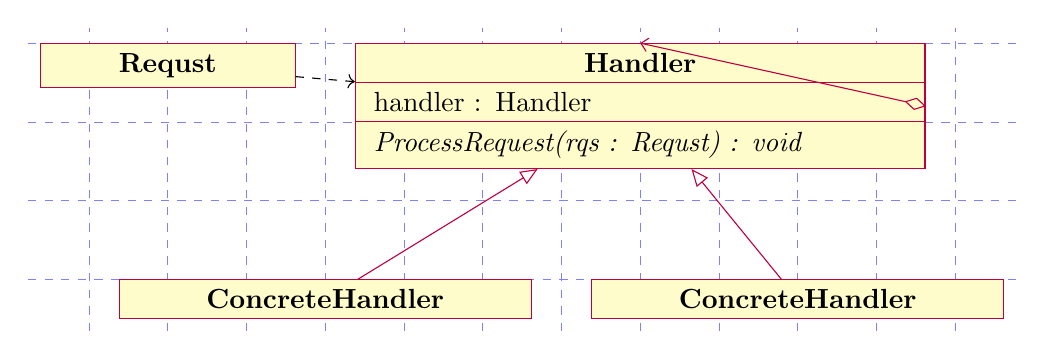
\begin{tikzpicture}[show background grid]
        \begin{class}[text width=3cm]{Requst}{0,0}
        \end{class}

        \begin{class}[text width=7cm]{Handler}{6, 0}
            \attribute{ handler : Handler }
            \operation[0]{ ProcessRequest(rqs : Requst) : void}
        \end{class}
        \aggregation{Handler.east}{}{}{Handler.north}
        \draw [dashed, ->] (Requst) -- (Handler);
        \begin{class}[]{ConcreteHandler}{2, -3}
            \inherit{Handler}
        \end{class}
        \begin{class}[]{ConcreteHandler}{8, -3}
            \inherit{Handler}
        \end{class}
        
    \end{tikzpicture}

\end{document}